\documentclass{beamer}

\usepackage[utf8]{inputenc}
\usepackage[english]{babel}
\usepackage{amsmath}
\usepackage{amssymb}
\usepackage{amsthm}
\usepackage{commath}
\usepackage{mathtools}
\usepackage{faktor}
\usepackage{color}
\usepackage{graphicx}
\usepackage{multirow}
\usepackage{array}
\usepackage{multirow}
\usepackage{breqn}
\usepackage[adversary, operators, sets, primitives, notions, probability, advantage, ff]{cryptocode}
\usepackage{todonotes}
\usepackage{tikz-cd}
\usepackage{hyperref}

\hypersetup{
    colorlinks,
    citecolor=black,
    %filecolor=black,
    linkcolor=black,
    urlcolor=blue
}

%\addtolength{\topmargin}{-.5in}
%\addtolength{\textheight}{0.5in}



\newtheorem{theorem}{Theorem}[section]
\newtheorem*{theorem*}{Theorem}
%\newtheorem{algorithm}[theorem]{Algoritmo}
%\newtheorem{claim}[theorem]{Claim}
%\newtheorem{conjecture}[theorem]{Congettura}
\newtheorem{corollary}[theorem]{Corollary}
\newtheorem{lemma}[theorem]{Lemma}
\newtheorem{problem}{Problem}[section]
\newtheorem{proposition}[theorem]{Proposition}

\theoremstyle{definition}
\newtheorem{definition}{Definition}[section]
\newtheorem{example}[theorem]{Example}

\theoremstyle{remark}
\newtheorem*{remark}{Remark}
\newtheorem{assumption}{Assumption}[section]
\newtheorem*{oss}{Observation}



\newcommand{\zdv}{\adversary{Z}}
\newcommand{\Fun}{\mathcal{F}}
\newcommand{\keygen}{\mathsf{KeyGen}}
\newcommand{\encaps}{\mathsf{Encaps}}
\newcommand{\decaps}{\mathsf{Decaps}}


\DeclareMathOperator{\lcm}{lcm}
\DeclareMathOperator{\Imm}{Im}
\DeclareMathOperator{\Dom}{Dom}
\DeclareMathOperator{\End}{End}
\DeclareMathOperator{\Hom}{Hom}
\DeclareMathOperator{\Aut}{Aut}
\DeclareMathOperator{\car}{char}
\DeclareMathOperator{\st}{\; |\;}
\DeclareMathOperator{\et}{\;\wedge\;}
\DeclareMathOperator{\tr}{Tr}
\DeclareMathOperator{\n}{N}
\DeclareMathOperator{\disc}{disc}
\DeclareMathOperator{\GL}{GL}


\newcommand{\N}{\mathbb{N}}
\newcommand{\Z}{\mathbb{Z}}
\newcommand{\Q}{\mathbb{Q}}
\newcommand{\R}{\mathbb{R}}
\newcommand{\C}{\mathbb{C}}
\newcommand{\F}{\mathbb{F}}
\newcommand{\Oc}{\mathcal{O}}
\newcommand{\Zn}[1]{\Z/#1\Z}
\newcommand{\ds}{\displaystyle}
\newcommand{\eps}{\varepsilon}



\usetheme{Frankfurt}
\useinnertheme{circles}
%\useoutertheme{miniframes}


\title{Isogeny-based Oblivious Transfer Protocols}
\author{Riccardo Zanotto}
\date{\today}


\begin{document}
    
    \createprocedureblock{myproc}{center, boxed}{}{}{}
    
    \begin{frame}
        \maketitle
    \end{frame}

    \begin{frame}
        \frametitle{Contents}
        \tableofcontents
    \end{frame}

    \section{Oblivious transfer}
    \begin{frame}
        \frametitle{What is oblivious transfer?}
        
        \begin{center}
        \begin{bbrenv}{A}
            
            \begin{bbrbox}[name=OT, namepos=middle, minheight=2cm]
                
            \end{bbrbox}
            \bbrmsgto{top={$(m_0,m_1)$},fixedoffset=2ex,length=1.5cm}
            \bbrmsgtxt[xshift=1.5cm]{
\includegraphics[height=5cm]{images/Alice}}
            
            \bbrqryfrom{top=$\sigma$,fixedoffset=2ex,length=1.5cm}
            \bbrqryto{top=$m_\sigma$,fixedboffset=2ex,length=1.5cm}
            \bbrqrytxt[]{
\includegraphics[height=5cm]{images/Bob}}
            
        \end{bbrenv}
        \end{center}        
    \end{frame}

    \begin{frame}
        \frametitle{Multi-party computation}
        
        \centering
        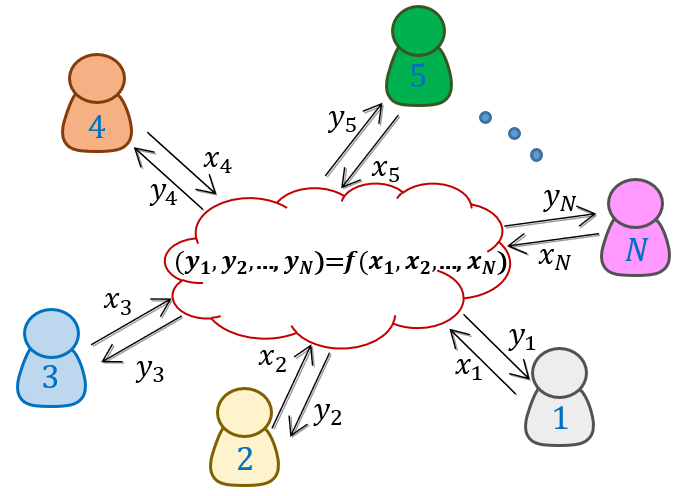
\includegraphics[width=0.9\textwidth]{images/MPC}
    \end{frame}

    \begin{frame}
        \frametitle{Why?}
        \begin{block}{Why MPC?}
            MPC studies the task of \emph{computing on private data}; sillier and serious examples:
            \begin{itemize}
                \item Deciding who is richer between two people without revealing their total worth.
                \item Running auctions with secret bidding.
                \item Distributed voting.
                \item Threshold signatures or decryptions.
                \item Running machine learning models on sensitive information, like X-ray pictures.
            \end{itemize}
        \end{block}
    

    \end{frame}

    \begin{frame}
        \frametitle{Why?}
        \begin{block}{Why OT?}
            Oblivious transfer is defined by a very simple function: $$f((m_0,m_1),\sigma)=(\lambda,m_\sigma)$$
            It can be used as a \emph{building block} of any MPC protocol, via the GMW construction (or \emph{garbled circuits}).
        \end{block}
    
        \pause
        \begin{block}{What do we want from OT?}
            \begin{itemize}
                \item Efficiency: for MPC we require many OTs; ususally they use public key cryptography (slow), so we need to keep low the number of rounds and the public key operations.
                \item Security: since the OTs can be run in parallel, we want privacy for concurrent executions and compositions.
            \end{itemize}
        \end{block}
    
    \end{frame}

    \begin{frame}
        \frametitle{Diffie-Hellman}
        
        \begin{block}{A key-exchange}
            Diffie-Hellman is a \emph{key-exchange} protocol, meaning that the two parties Alice and Bob can communicate over a public channel and end up with some shared secret value.
            Usually it takes place in the moltiplicative group $\F_p^\ast$, with generator $g$.
        \end{block}
        
        \begin{center}
            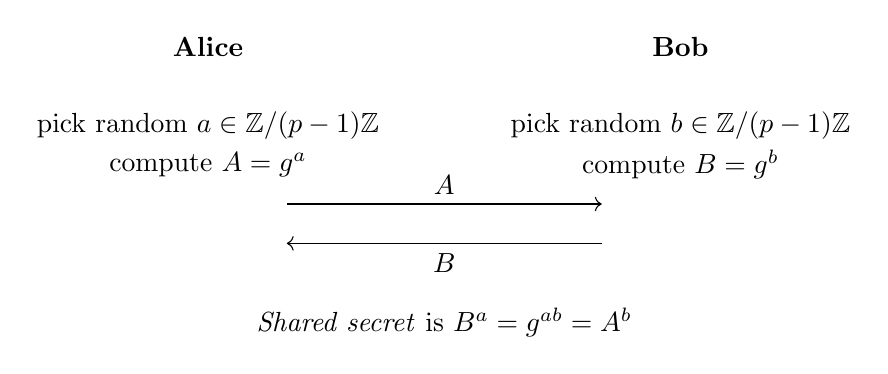
\begin{tikzpicture}
            \node at (0,0) {\bf Alice};
            \node at (6,0) {\bf Bob};
            \node at (0,-1) {pick random $a\in\Zn{(p-1)}$};
            \node at (0,-1.5) {compute $A=g^a$};
            \node at (6,-1) {pick random $b\in\Zn{(p-1)}$};
            \node at (6,-1.5) {compute $B=g^b$};
            \draw[->]
            (1,-2) to node[auto] {$A$} (5,-2);
            \draw[->] (5,-2.5) to node[auto] {$B$} (1,-2.5);
            \node at (3,-3.5) {\emph{Shared secret} is \alert{$B^a=g^{ab}=A^b$}};
            \end{tikzpicture}
        \end{center}
    \end{frame}

    \begin{frame}
        \frametitle{Diffie-Hellman}
        \begin{block}{Security}
            The shared value between Alice and Bob is actually secret, because an attacker can only get the public keys $A$ and $B$. In order to compute $g^{ab}$ he needs one of $a,b$.
            
            Computing a secret $x$ from the value $g^x\pmod p$ is the \emph{discrete logarithm problem}. There are no known polynomial algorithms to solve it, the best is GNFS which is subexponential.
        \end{block}
    
        \pause
        \begin{block}{ECDH}
            Notice that $DH$ can be done in any abelian group; in 1980s Koblitz thought ``why don't we use the group of points on an elliptic curve?", and now our phones perform thousands of point additions whenever we open Facebook.
        \end{block}
    \end{frame}

    \begin{frame}
        \frametitle{The simplest OT}
        
        \begin{center}
            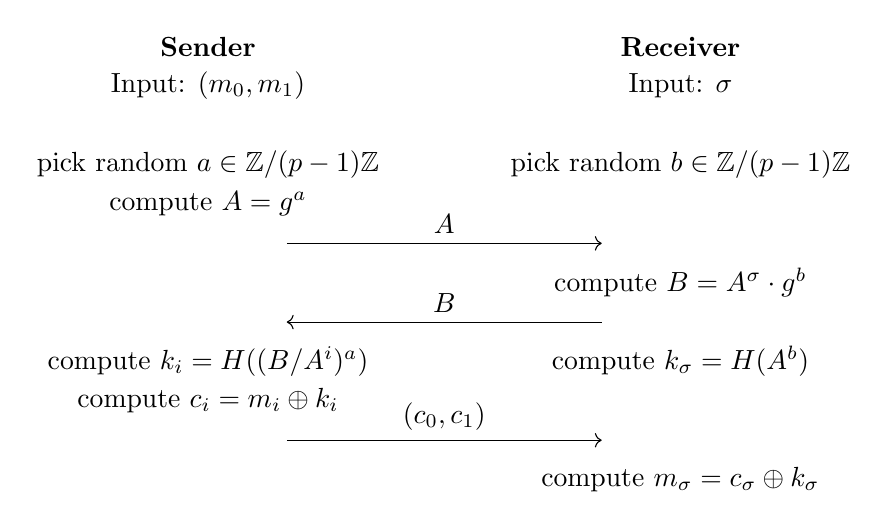
\begin{tikzpicture}
            \node at (0,0) {\bf Sender};
            \node at (6,0) {\bf Receiver};
            \node at (0,-0.5) {Input: $(m_0,m_1)$};
            \node at (6,-0.5) {Input: $\sigma$};
            \node at (0,-1.5) {pick random $a\in\Zn{(p-1)}$};
            \node at (0,-2) {compute $A=g^a$};
            \node at (6,-1.5) {pick random $b\in\Zn{(p-1)}$};          
            \draw[->] (1,-2.5) to node[auto] {$A$} (5,-2.5);
            \node at (6,-3) {compute $B=A^\sigma\cdot g^b$};
            \draw[->] (5,-3.5) to node[above] {$B$} (1,-3.5);
            \node at (0,-4) {compute $k_i=H((B/A^i)^a)$};
            \node at (6,-4) {compute $k_\sigma=H(A^b)$};
            \node at (0,-4.5) {compute $c_i=m_i\oplus k_i$};
            \draw[->] (1,-5) to node[above] {$(c_0,c_1)$} (5,-5);
            \node at (6,-5.5) {compute $m_\sigma=c_\sigma\oplus k_\sigma$};
            \end{tikzpicture}
        \end{center}
    \end{frame}

    \begin{frame}
        \frametitle{The simplest OT}
        
        \begin{block}{Who?}
            Proposed by Chou and Orlandi in 2015.
        \end{block}
    
        \begin{block}{Why?}
            It is very efficient: the picture is simplified, but it's a $k$-out-of-$n$ OT using DH over elliptic curves (in Edwards model).
            
            It is secure, since the receiver can't know both the values $g^{ab}g^{a^2(\sigma-i)}$; otherwise he could compute the value $a$, thus solving a discrete logarithm.
        \end{block}
    \end{frame}


    \begin{frame}
        \frametitle{The simplest OT}
        
        \begin{block}{Why not?}
            \begin{itemize}[<+->]
                \item Uses Diffie-Hellman: Shor's quantum algorithm solves the discrete logarithm problem in polynomial time. If we want security in a world with quantum computers, we need new cryptography.
                \item Wrong security proof: the proofs for MPC protocols are done in the Universal Composability framework and require many details; other cryptographers noticed that the authors missed some of them. There seems to be no way of fixing the proof.
            \end{itemize}
        \end{block}
    \end{frame}


    \section{Isogeny-based cryptography}
    
    \begin{frame}
        \frametitle{Post-quantum cryptography}
        
        \begin{block}{The problem}
            In 1994 Shor found a quantum polynomial algorithm for \emph{order finding}. With this, it is possible to solve dicrete logarithms in any abelian group and to factor large integers.
            
            Most of public key cryptography is then broken (RSA, DH, ECDH).
        \end{block}
    
        \pause
        \begin{block}{The solution}
            In 2016 NIST started a competition to find new \emph{post-quantum} public key primitives. The proposals are based on:
            \begin{itemize}
                \item Lattices
                \item Codes
                \item Multivariate equation
                \item \color<3->{red}{Supersingular isogenies}
            \end{itemize}
        \end{block}
    \end{frame}

    \begin{frame}
        \frametitle{Elliptic curves}
        
        \begin{definition}
            An \emph{elliptic curve} $E$ \emph{over} $K$ is a smooth projective curve of genus $1$, with a given $K$-rational point.
        \end{definition}
    
        \begin{block}{For cryptographers}
            An elliptic curve $E$ is a Weierstrass equation $$y^2=x^3+ax+b$$ where $4a^3+27b^2\neq0$; don't forget the point at infinity!
        \end{block}
    
        \begin{theorem}
            Let $E$ be an elliptic curve over $K$; then $E(K)$ has an abelian group structure $\oplus$, with neutral element the point at infinity.
        \end{theorem}
    \end{frame}

    \begin{frame}
        \frametitle{The group law}
        \begin{center}
            \begin{tikzpicture}[domain=-2.4566:4,samples=100,yscale=1/2]
            \draw plot (\x,{sqrt(\x*\x*\x-4*\x+5)});
            \draw plot (\x,{-sqrt(\x*\x*\x-4*\x+5)});
            
            \draw[thin,gray,-latex] (0,-7) -- (0,7);
            \draw[thin,gray,-latex] (-3,0) -- (4,0);
            \draw (-3,1) -- (4,8/3+3);
            \begin{scope}[every node/.style={draw,circle,inner sep=1pt,fill},cm={1,2/3,0,0,(0,3)}]
            \node at (-2.287980,0) {};
            \node at (-0.535051,0) {};
            \node at (3.267475,0) {};
            \end{scope}
            \begin{scope}[every node/.style={yshift=0.3cm},cm={1,2/3,0,0,(0,3)}]
            \node at (-2.287980,0) {$P$};
            \node at (-0.535051,0) {$Q$};
            \node at (3.267475,0) {$R$};
            \end{scope}
            
            \draw[dashed] (3.267475,3.267475*2/3+3) -- (3.267475,-3.267475*2/3-3) 
            node[draw,circle,inner sep=1pt,fill] {}
            node[xshift=-0.1cm,anchor=east] {$P\oplus Q$};
            \end{tikzpicture}
        \end{center}
    \end{frame}

    \begin{frame}
        \frametitle{Isogenies}
        
        \begin{definition}
            Let $E_1$ and $E_2$ be elliptic curves, with points at infinity $O_1,O_2$. An \emph{isogeny} is a morphism of curves $\phi:E_1\to E_2$ such that $\phi(O_1)=O_2$.
        \end{definition}
    
        \begin{theorem}
            Let $\phi:E_1 \to E_2$ be a non-constant isogeny. Then $\phi$ induces a surjective group homomorphism $E_1(\bar K)\to E_2(\bar K)$ with finite kernel.
            
            Moreover, separable isogenies are in bijections with finite subgroups of $E_1$.
        \end{theorem}
    
        \begin{block}{Vélu's formula}
            Given a subgroup $G<E(K)$ of an elliptic curve defined over $K$, there is a formula that in time $O(\# G)$ computes the corresponding isogeny and the codomain curve.
        \end{block}
    \end{frame}

    \begin{frame}
        \frametitle{Special isogenies}
        
        \begin{example}
            Multiplication-by-m
        \end{example}
    
        \begin{theorem}
            Dual isogeny
        \end{theorem}
    \end{frame}

    \begin{frame}
        \frametitle{Elliptic curves over finite fields}
        
        \begin{definition}
            Frobenius endomorphism
        \end{definition}
    
        \begin{theorem}
            Let $E/\F_q$ be an elliptic curve and $\pi$ its Frobenius endomorphism. Then there exists $t\in\Z$ such that $$\pi^2-t\pi+q=0.$$
            
            Moreover, $\# E(\F_q) = q+1-t$ with $|t|\le2\sqrt q$.
        \end{theorem}
    \end{frame}

    \begin{frame}
        \frametitle{Supersingular elliptic curves}
        
        \begin{theorem}
            Let $E/K$ be an elliptic curve, with $\car K=p$. The following are equivalent:
            \begin{enumerate}
                \item $E[p^r]=\{O\}$ for some (all) $r\ge1$.
                \item The dual isogeny $\hat\pi$ is inseparable.
                \item The map $[p]:E\to E$ is purely inseparable and $j(E)\in\F_{p^2}$.
                \item $\End(E)$ is a maximal order in a quaternion algebra.
            \end{enumerate}
            If any of these properties hold, we say that $E$ is \emph{supersingular}; otherwise $E$ is said to be \emph{ordinary}.
        \end{theorem}
    \end{frame}

    \begin{frame}
        \frametitle{The CM action}
        
        \begin{definition}
            Let $\Oc$ be an order in an imaginary quadratic field $K$, and denote by $Ell_q(\Oc)$ the set of $\F_q$-isomorphism classes of elliptic curves with \emph{complex multiplication} by $\Oc$, i.e. with $\End_{\F_q}(E)=\Oc$.
        \end{definition}
        
        \begin{theorem}
            Let $\F_q$ be a finite field and $\Oc\subset\Q(\sqrt{-D})$ an order in a quadratic imaginary field. Assume $Ell_q(\Oc)$ is non empty; then there is a free and transitive action given by
            \begin{align*}
            Cl(\Oc)\times Ell_q(\Oc) & \to  Ell_q(\Oc)\\
            (\mathfrak{a}, E) & \mapsto  E/E[\mathfrak{a}]
            \end{align*}
        \end{theorem}
    
    \end{frame}

    \begin{frame}
        \frametitle{CM graphs}
        
        \begin{center}
            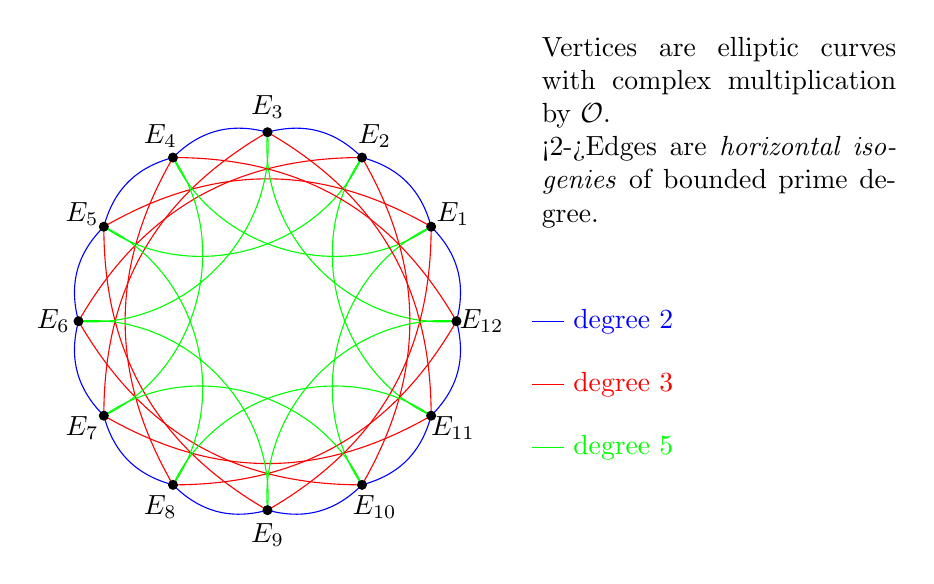
\begin{tikzpicture}[scale=0.8]
            \begin{scope}
            \def\crater{12}
            \def\jumpa{-8}
            \def\jumpb{9}
            \def\diam{3cm}
            
            \foreach \i in {1,...,\crater} {
                \uncover<2->{\draw[blue] (360/\crater*\i : \diam) to[bend right] (360/\crater*\i+360/\crater : \diam);}
                \uncover<3->{\draw[red] (360/\crater*\i : \diam) to[bend right] (360/\crater*\i+\jumpa*360/\crater : \diam);}
                \uncover<4->{\draw[green] (360/\crater*\i : \diam) to[bend right=50] (360/\crater*\i+\jumpb*360/\crater : \diam);}
            }
            \foreach \i in {1,...,\crater} {
                \draw[fill] (360/\crater*\i: \diam) circle (2pt) +(360/\crater*\i: 0.4) node{$E_{\i}$};
            }
            \end{scope}
            \begin{scope}[xshift=4.2cm]
            \draw (0,3) node[anchor=west] {\parbox{4.5cm}{%
                    Vertices are elliptic curves with complex
                        multiplication by $\Oc$.\\
                    \uncover<2->{Edges are \emph{horizontal isogenies} of
                        bounded prime degree.}  }};
            
            \uncover<2->{\draw[blue] (0,0) -- (0.5,0)
                (0.5,0) node[anchor=west] {degree $2$};}
            \uncover<3->{\draw[red] (0,-1) -- (0.5,-1) (0.5,-1)
                node[anchor=west] {degree $3$};}
            \uncover<4->{\draw[green]
                (0,-2) -- (0.5,-2) (0.5,-2) node[anchor=west] {degree $5$};}
            
            \end{scope}
            \end{tikzpicture}
        \end{center}
    
    \end{frame}

    \begin{frame}
        \frametitle{Hard homogeneous spaces}
        
        \begin{definition}
            A hard homogeneous space consists of a finite abelian group $G$ acting freely and transitively on a set $X$.
            
            The following tasks are required to be easy (i.e. polynomial-time):
            \begin{enumerate}
                \item Computing group operations in $G$.
                \item Computing the action of a group element $g\in G$ on some $x\in X$.
            \end{enumerate}
            
            The following tasks are instead required to be hard (i.e. not polynomial-time):
            \begin{enumerate}
                \setcounter{enumi}{2}
                \item Vectorization: given $x,x'\in X$, find $g\in G$ such that $g\star x=x'$.
                \item Parallelization: given $x,x',y\in X$ with $g\star x=x'$, compute $y'\in X$ such that $g\star y=y'$.
            \end{enumerate}
        \end{definition}
        
    \end{frame}


    \begin{frame}
        \frametitle{A HHS from complex multiplication}
    
    \end{frame}


    \begin{frame}
        \frametitle{The CSIDH protocol}
        
        \begin{block}{}
            \textbf{Setup}: A prime $p=4\ell_1\cdots\ell_n-1$, where $\ell_i$ are small distinct odd primes; $E_0:y^2=x^3+x$ is the base supersingular elliptic curve with $\Oc:=\End_p(E_0)=\Z[\pi]$. Fix also a parameter $m$.
            
            \textbf{Key generation}: Sample a tuple of integers $(e_1,\dots,e_n)$ from $\{ -m,\dots,m \}^n$. This tuple corresponds to the ideal $[\mathfrak{a}] = \prod [\mathfrak{l}_i]^{e_i}$ of $Cl(\Oc)$, where $\mathfrak{l}_i=(\ell_i, \pi-1)$. The public key is the $A$ coefficient of the curve $[\mathfrak{a}]E_0:y^2=x^3+Ax^2+x$ in Montgomery form.
            
            \textbf{Key exchange}: Suppose Alice and Bob have key pairs $([\mathfrak{a}], A)$ and $([\mathfrak{b}], B)$. When receiving $B$ from Bob, Alice checks the validity of this public key and then computes the curve $[\mathfrak{a}]E_B$. Bob does the same and computes $[\mathfrak{b}]E_A$. The shared secret is the Montgomery coefficient $S$ of the curve $[\mathfrak{a}][\mathfrak{b}]E_0=[\mathfrak{b}][\mathfrak{a}]E_0$ written as $y^2=x^3+Sx^2+x$.
        \end{block}
    
    \end{frame}

    \begin{frame}
        \frametitle{Quantum security of CSIDH}
    
    \end{frame}


    
    
    \section{Security definitions}
    
    \begin{frame}
        \frametitle{}
    
    \end{frame}

    \begin{frame}
        \frametitle{}
    
    \end{frame}
    
    \begin{frame}
        \frametitle{Universal composability}
    \end{frame}

    
    \section{The Explicit Isogeny model}
        
    \begin{frame}
        \frametitle{Our result}
    \end{frame}

\end{document}